% Options for packages loaded elsewhere
\PassOptionsToPackage{unicode}{hyperref}
\PassOptionsToPackage{hyphens}{url}
%
\documentclass[
]{article}
\usepackage{amsmath,amssymb}
\usepackage{lmodern}
\usepackage{ifxetex,ifluatex}
\ifnum 0\ifxetex 1\fi\ifluatex 1\fi=0 % if pdftex
  \usepackage[T1]{fontenc}
  \usepackage[utf8]{inputenc}
  \usepackage{textcomp} % provide euro and other symbols
\else % if luatex or xetex
  \usepackage{unicode-math}
  \defaultfontfeatures{Scale=MatchLowercase}
  \defaultfontfeatures[\rmfamily]{Ligatures=TeX,Scale=1}
\fi
% Use upquote if available, for straight quotes in verbatim environments
\IfFileExists{upquote.sty}{\usepackage{upquote}}{}
\IfFileExists{microtype.sty}{% use microtype if available
  \usepackage[]{microtype}
  \UseMicrotypeSet[protrusion]{basicmath} % disable protrusion for tt fonts
}{}
\makeatletter
\@ifundefined{KOMAClassName}{% if non-KOMA class
  \IfFileExists{parskip.sty}{%
    \usepackage{parskip}
  }{% else
    \setlength{\parindent}{0pt}
    \setlength{\parskip}{6pt plus 2pt minus 1pt}}
}{% if KOMA class
  \KOMAoptions{parskip=half}}
\makeatother
\usepackage{xcolor}
\IfFileExists{xurl.sty}{\usepackage{xurl}}{} % add URL line breaks if available
\IfFileExists{bookmark.sty}{\usepackage{bookmark}}{\usepackage{hyperref}}
\hypersetup{
  pdftitle={Moralizing high gods in cross-cultural datasets systematically underestimate the evidence for supernatural punishment},
  pdfauthor={Indigenous Religions Lab, feat. Ryan McKay},
  hidelinks,
  pdfcreator={LaTeX via pandoc}}
\urlstyle{same} % disable monospaced font for URLs
\usepackage[margin=1in]{geometry}
\usepackage{longtable,booktabs,array}
\usepackage{calc} % for calculating minipage widths
% Correct order of tables after \paragraph or \subparagraph
\usepackage{etoolbox}
\makeatletter
\patchcmd\longtable{\par}{\if@noskipsec\mbox{}\fi\par}{}{}
\makeatother
% Allow footnotes in longtable head/foot
\IfFileExists{footnotehyper.sty}{\usepackage{footnotehyper}}{\usepackage{footnote}}
\makesavenoteenv{longtable}
\usepackage{graphicx}
\makeatletter
\def\maxwidth{\ifdim\Gin@nat@width>\linewidth\linewidth\else\Gin@nat@width\fi}
\def\maxheight{\ifdim\Gin@nat@height>\textheight\textheight\else\Gin@nat@height\fi}
\makeatother
% Scale images if necessary, so that they will not overflow the page
% margins by default, and it is still possible to overwrite the defaults
% using explicit options in \includegraphics[width, height, ...]{}
\setkeys{Gin}{width=\maxwidth,height=\maxheight,keepaspectratio}
% Set default figure placement to htbp
\makeatletter
\def\fps@figure{htbp}
\makeatother
\setlength{\emergencystretch}{3em} % prevent overfull lines
\providecommand{\tightlist}{%
  \setlength{\itemsep}{0pt}\setlength{\parskip}{0pt}}
\setcounter{secnumdepth}{5}
\ifluatex
  \usepackage{selnolig}  % disable illegal ligatures
\fi
\newlength{\cslhangindent}
\setlength{\cslhangindent}{1.5em}
\newlength{\csllabelwidth}
\setlength{\csllabelwidth}{3em}
\newenvironment{CSLReferences}[2] % #1 hanging-ident, #2 entry spacing
 {% don't indent paragraphs
  \setlength{\parindent}{0pt}
  % turn on hanging indent if param 1 is 1
  \ifodd #1 \everypar{\setlength{\hangindent}{\cslhangindent}}\ignorespaces\fi
  % set entry spacing
  \ifnum #2 > 0
  \setlength{\parskip}{#2\baselineskip}
  \fi
 }%
 {}
\usepackage{calc}
\newcommand{\CSLBlock}[1]{#1\hfill\break}
\newcommand{\CSLLeftMargin}[1]{\parbox[t]{\csllabelwidth}{#1}}
\newcommand{\CSLRightInline}[1]{\parbox[t]{\linewidth - \csllabelwidth}{#1}\break}
\newcommand{\CSLIndent}[1]{\hspace{\cslhangindent}#1}

\title{Moralizing high gods in cross-cultural datasets systematically underestimate the evidence for supernatural punishment}
\author{Indigenous Religions Lab, feat. Ryan McKay}
\date{}

\begin{document}
\maketitle
\begin{abstract}
Many have theorized from cross-cultural and evolutionary perspectives about the interacting roles between punitive, moralizing gods and social complexity. The premise of this theorizing assumes a positive association between the presence of moralizing gods and high levels of social complexity. An influential source of evidence for this premise is the Standard Cross-Cultural Sample (SCCS), specifically with its moralizing \emph{high god} variable as the outcome of interest. In this paper, we discuss how the high god variable is coded. We then show why, based on this coding criteria, the SCCS systematically underestimates our outcome of interest (whether a punitive, moralizing god is present in a given culture) because it filters cases based on a theoretically irrelevant criterion (whether a god is a creator deity, regardless of its power or omniscience). Based on existing evidence that \emph{does} include both moralizing gods and moralizing \emph{high} gods, we then show that this problem of false negatives in the ethnographic record is not randomly distributed across levels of social complexity. Instead, these false negatives are likely biased in a way that favors more false negatives at lower levels of social complexity, favoring a spurious positive association between presence of moralizing gods and social complexity. We then argue that this apparent bias is likely strengthened by the historical context in which the data were generated in this first place. We therefore question the premise that punitive, moralizing gods are positively associated with high social complexity, and argue that the currently available sources of cross-cultural data tend to underestimate the prevalence of moralizing gods in small-scale societies.
\end{abstract}

\section{Introduction}

Many have theorized, from cross-cultural and evolutionary perspectives, about how moralizing and punitive \emph{Big Gods} relate to social complexity. A popular working narrative, which we refer to as the \emph{Big Gods narrative}, often goes as follows. During most of our evolutionary history, humans followed animistic religious traditions, anthropomorphizing their social and natural worlds with spirits, demons, and witches. Echoing late-nineteenth and early-twentieth century theories of animistic religions among small-scale societies (Tylor 1871), these ``ancestral religions did not have a clear moral dimension'' (Norenzayan 2015:127). In the past 12,000 years or so, however, people started to believe in so-called \emph{Big Gods}: powerful deities who monitor human behavior, care about upholding moral rules, and punish rule violators (Norenzayan 2015; Norenzayan et al. 2016; Jackson et al. 2021). Whereas gods in modern small-scale and prehistorical societies tend to be ``weak, whimsical, and not particularly moral'' (Henrich 2020), morally concerned ``super-punishers'' are associated with complex, large-scale societies because they motivate an expansion of cooperation that kin selection and reciprocity cannot sustain (Henrich and Muthukrishna 2021:24; see also Norenzayan et al. 2016). Hence, the Big Gods narrative implies a positive association between the presence of moralizing, punitive gods and social complexity.

Many studies supplying the anthropological evidence for a positive association between moralizing supernatural punishers have done so with the Standard Cross-Cultural Sample (SCCS), a cross-cultural survey of 186 societies (Snarey 1996; Roes and Raymond 2003; e.g., Johnson 2005; Norenzayan et al. 2016).\footnote{Anthropology is a field that has been motivated to understand humans in the broadest sense for more than a century, and the usefulness of this dataset for doing so should not be underestimated. We therefore caution against viewing our critical discussion as a general critique of the SCCS, although a fair amount of skepticism of its results is always warranted -- as we will demonstrate in this paper.} In the SCCS, there is one variable, V237, that measures the presence vs.~absence of moralizing \emph{high gods} (MHGs) and a handful of variables that measure social complexity (e.g., V238, which is the number of jurisdictional hierarchies). To use a widely circulated example, there are 167 societies with complete data on V237 (presence/absence of MHGs) and V238 (number of jurisdictional hierarchies), and the proportion of MHGs present generally increases at each level of jurisdictional hierarchies (figure \ref{fig:standardSCCS}). The SCCS is not the only source of cross-cultural data available on social complexity and moralizing high gods. Indeed, the coding criteria for the MHG variable is identical to the one in Swanson (1964), which examines moralizing gods and social complexity among 60 societies (see also Peregrine 1996). Swanson's dataset, like the SCCS, shows a similar association between MHGs and social complexity (figure \ref{fig:mhgPlot}).

\begin{figure}
\centering
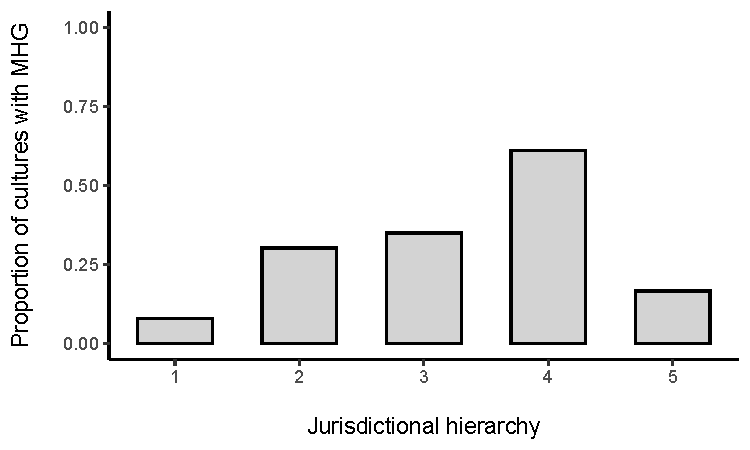
\includegraphics{mhg-writeup_files/figure-latex/standardSCCS-1.pdf}
\caption{\label{fig:standardSCCS}Proportion of MHGs in each level of social complexity, as measured by the number of jurisdictional hierarchies, among 167 cultures in the SCCS. Note that this is from the latest version of the SCCS, available at D-PLACE, and it differs slightly when compared to the key results in other works, such as Roes and Raymond (2003).}
\end{figure}

\begin{figure}
\centering
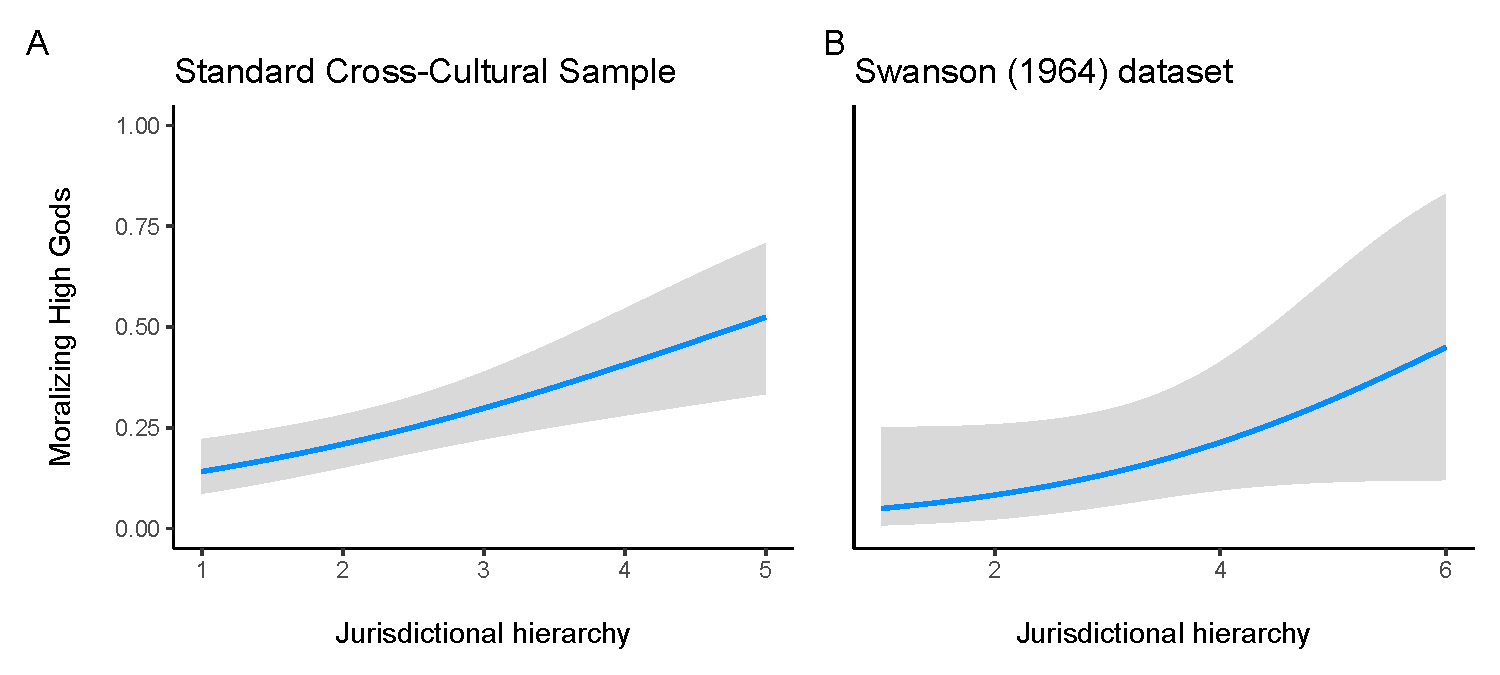
\includegraphics{mhg-writeup_files/figure-latex/mhgPlot-1.pdf}
\caption{\label{fig:mhgPlot}Logistic regression models showing an increased probability of a MHG present (y-axis) along increasing levels of social complexity, measured by the number of jurisdictional hierarchies (x-axis). Model results are based on coded data among cultures in the SCCS (panel A) and in the Swanson dataset (panel B).}
\end{figure}

The observation that MHGs and social complexity levels are positively associated in the cross-cultural data has provided much of the fuel for the Big Gods narrative. Indeed, when discussing the anthropological evidence for the Big Gods narrative, the Big Gods term is frequently used as a convenient and interchangeable shorthand for the MHGs in the SCCS (e.g., sect. 3 in Norenzayan et al. 2016). The problem with using MHGs and Big Gods interchangeably, however, is that the MHG variable is restrictively defined in a way that leads to a high false negative rate when attempting to detect the presence of moralizing gods. (As we will discuss further below, by \emph{false negatives} we mean an inference that incorrectly attributes the absence of a characteristic of interest that is truly present.)

\section{Moralizing gods, moralizing high gods: What's the difference?}

In a classic paper that helped shape the Big Gods narrative, Roes and Raymond (2003) investigated MHGs in the SCCS as a measure of what they refer to as \emph{moralizing gods}. Their concept of moralizing gods (MGs) is broadly characterized by supernatural punishment, resembling the Big Gods concept: they are gods who ``tell people what they should and should not do'' (p.~127), ``induce society members to cooperate with one another,'' and ``impose {[}their moral rules{]} with authority'' (p.~135). These MGs (and subsequently, Big Gods) are, in other words, a theoretical construct that MHGs are meant to measure in the cross-cultural and ethnographic data.

Hence, we have three loosely connected terms to work with in our analysis: Big Gods, moralizing gods (MGs), and moralizing high gods (MHGs). It is perhaps intuitive to refer to these terms interchangeably, because Big Gods and MHGs seem, in many ways, like prototypical representations of a deity such as the Christian God: ``a single, all-powerful creator'' that is actively concerned about human morality (Peoples and Marlowe 2012:253).

It is not obvious, however, that MHGs are theoretically relevant to Big Gods or its closely related concept of broadly moralizing gods (MGs), because \emph{high} gods are distinguished from all other gods by their status as a \emph{creator} deity. The \emph{high god} variable, both in the SCCS and in Swanson (1964), is defined as ``a spiritual being who is believed to have created all reality and/or to be its ultimate governor,'' and ``includes spirits whose sole act was to create the other spirits who, in turn, produced the natural world'' (p.~210). Non-missing data in the high gods variable can take on one of four categorical values: (1) \emph{absent}, (2) \emph{otiose}, (3) \emph{active, but not supporting morality}, and (4) \emph{active, supporting morality} (Swanson 1964; Murdock and White 2006; Kirby et al. 2016).

We can therefore represent the coding decisions for presence vs.~absence of MHGs as a two-step decision tree: First, did a god create all of reality and/or control the natural world? Second, and given that a god met the first condition, does that god care about morality? A society is coded as having a MHG present if, and only if, both of these criteria are met.

MGs who mete out supernatural punishment are a theoretical construct that MHGs are meant to measure. While the theoretical relevance of the second criterion to supernatural punishment is clear, the relevance of the first criterion, which filters \emph{all cases that can be considered for the second criterion}, is not clearly relevant to supernatural punishment.\footnote{As we will discuss further, its similarity to the Christian God might even reflect the historical contexts that shaped the discourse around moralizing gods in the twentieth century (see also Purzycki and McKay, forthcoming).} This way of defining MHGs as a subset of creator MGs seems to clash with popular uses of the Big Gods concept, which seems more akin to a broadly punitive MG concept that MHGs are meant to measure. (Notice, for example, that the criteria for MHGs do not include criteria such as omniscience or a wide scope of gods' concerns, which are sometimes used to differentiate Big Gods from weak and whimsical gods.)

\subsection{Detecting moralizing gods in the ethnographic record: A problem of false negatives}

This is not simply an academic quibble about definitions; these differences in definitions have real consequences on the cross-cultural data that has shaped the Big Gods narrative and subsequent discussions (e.g., Beheim et al. 2019; Whitehouse et al. 2021). Even if we assumed that every ethnographer was perfectly reliable in his or her interpretation of a cultural institution,\footnote{This is, of course, not a safe assumption, and we will directly addess this further below.} the arbitrary filtering criteria that sits at the first step of coding presence/absence of MHGs -- does a culture have a creator deity? -- is bound to systematically generate false negatives in our cross-cultural data by excluding MGs who are not creator deities. If a culture has a punitive MG who motivates cooperation, but that MG neither created the world nor governs its everyday occurrences, then that culture's MHG data point is coded as ``absent.''

To illustrate, consider the following account of the Orokaiva (Schwimmer 1973):

\begin{quote}
If the Orokaiva, by and large, order their lives by the same moral principles, they would explain this by their common belief in certain demigods whom they all regard as their ancestors and as sources of authority, and who created certain institutions embodying moral norms to which they all subscribe. Not only do they obey the precepts of these demi-gods, they also re-enact their feats in ritual and identify with them during ceremonies, and in many of their regular expressive activities (p.~51).
\end{quote}

The Orokaiva appear to attribute their moral order to these demi-gods, who are both authoritative and responsible for institutions with moral significance. Nevertheless, the Orokaiva are coded, both in the SCCS and in Swanson's data, as lacking a MHG.\footnote{While it is not immediately relevant to our point in this section, it is worth pointing out that the Orokaiva are also coded as having one jurisdictional hierarchy, i.e., on the low complexity end of the V238 variable.} This might be technically true, but they do not lack MGs. Indeed, while Swanson (like the SCCS) codes the Orokaiva as lacking a high god (and hence, lacking a MHG), he also codes them as having moralistic supernatural sanctions present.\footnote{These variables, which can be coded as present vs. absent, are specifically \emph{Active Ancestral Spirits}: Present -- aid or punish living humans, \emph{Supernatural Sanctions for Morality -- Effects on Health}, \emph{Supernatural Sanctions for Morality -- Effects on Experiences in the Afterlife}, and \emph{Supernatural Sanctions for Morality -- Other Effects}. The ``other effects'' in the last variable includes accidents and misfortunes, such as crop failure. See Swanson 1964, p. 211-213.}

A better (and more theoretically relevant) alternative would be a variable that is more broadly based on MGs, who can, like Big Gods, motivate moral behaviors through supernatural punishment threats (Schloss and Murray 2011; Johnson 2015; Watts et al. 2015; Singh, Kaptchuk, and Henrich 2021) and/or form the basis of supernatural appeals (Bendixen and Purzycki 2020; Fitouchi and Singh 2021). Comparing the prevalence of MGs based on this criteria vs.~MHGs, when the data are available, would allow us to begin roughly assessing how severe of a false negative problem this coding criteria actually creates. The SCCS unfortunately lacks an alternative variable on MGs -- a practical reason to use MHGs to measure presence/absence of MGs in the first place. However, in addition to the high gods variable, Swanson's data includes multiple variables on supernatural punishment based on moral concerns, which are not constrained by the high god's filtering criteria.

\subsection{Estimating the impact of false negatives from an existing dataset}

A broad pass at the literature can give us a hint about how much more common MGs are than the prevalence of MHGs would seem to suggest. Consider, for example, some recent cross-cultural datasets that include broader coding criteria for MGs (e.g., Boehm 2008; Watts et al. 2015; Peoples, Duda, and Marlowe 2016; Skoggard et al. 2020; Whitehouse et al. 2021). Collectively, these datasets, many of which include MGs and MHGs as separate variables, suggest that that MGs are quite common and MHGs are not (figure \ref{fig:comparedatasets}). In other words, the problem of correctly detecting MGs by measuring MHGs is a general problem of misclassification of a binary outcome, a general problem for signal detection in presence/absence data that is especially common in epidemiology (Duffy et al. 2004; Edwards et al. 2013). In this case, we want to detect the presence of an MG, and we generate false negatives when doing so by measuring MHGs.

\begin{figure}
\centering
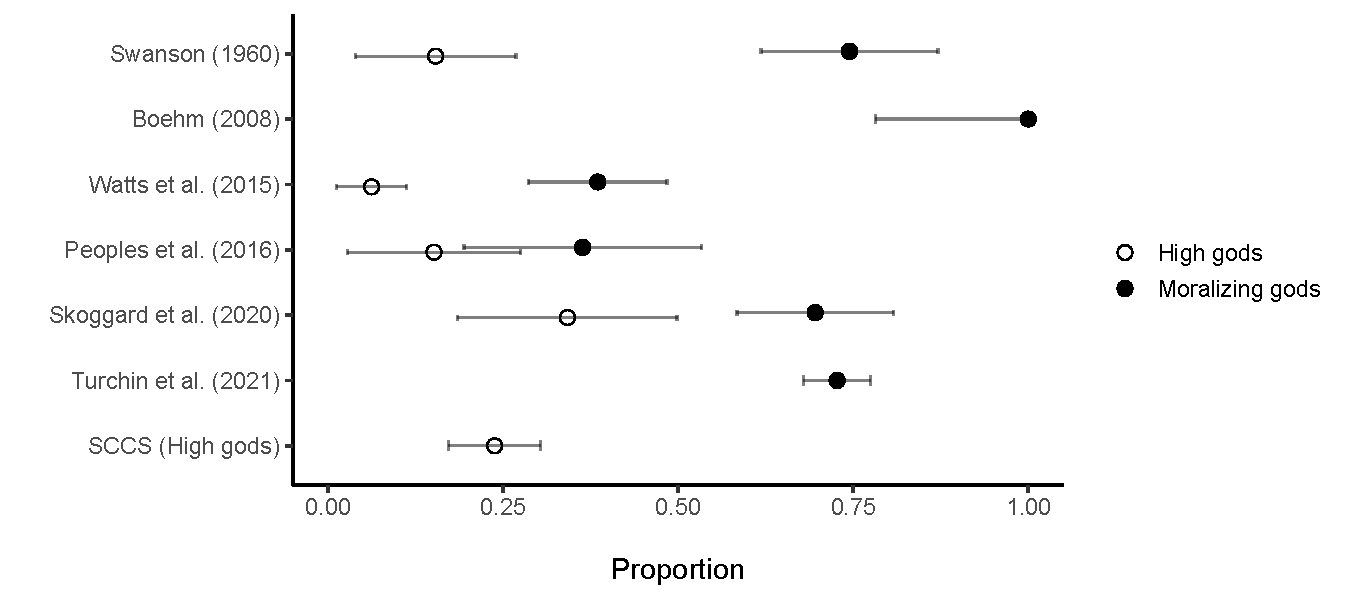
\includegraphics{mhg-writeup_files/figure-latex/comparedatasets-1.pdf}
\caption{\label{fig:comparedatasets}Proportion of MHGs present (open points) vs.~MGs present (closed points) in a sample of datasets that either include MHGs, MGs, or both. Error bars are bootstrapped 95\% CIs.}
\end{figure}

Many of these datasets in figure \ref{fig:comparedatasets} were also interested in social complexity, possibly allowing us to re-evaluate whether or not MGs are positively associated with levels of social complexity. However, most of them were either complicated by different levels of uncertainty over time (Whitehouse et al. 2021) or are restricted to a single subsistence strategy (Boehm 2008; Peoples, Duda, and Marlowe 2016), a single domain of supernatural punishment, such as weather (Skoggard et al. 2020), or a narrow region of interest (Watts et al. 2015). Of the available datasets in figure \ref{fig:comparedatasets}, the dataset in Swanson (1964) is our best available reference for making a simple, straightforward and cross-cultural assessment about how the documented prevalence of MHGs differs from the documented prevalence of MGs along different levels of social complexity.

When we group the cultures from Swanson's dataset by social complexity level\footnote{We refer to this variable as jurisdictional levels for consistency, but here and in the figures above, the Swanson dataset measures social complexity with the \emph{number of sovereign organizations} variable. This is similar to the jurisdictional levels variable (V238) in the SCCS, but is coded with up to six, rather than five, organizations. We focus on jurisdictional levels instead of population size because, as discussed in the Introduction, this variable is commonly used in the literature to measure social complexity.} and count up the number of MGs vs.~MHGs present vs.~absent, we see that many MHGs are absent among lower complexity levels -- consistent with the idea that higher social complexity is associated with MHGs. Many MGs are present among lower complexity levels, however, and proportional to the number of cultures sampled at each level of complexity, MGs appear to be generally widespread (figure \ref{fig:compareSwanson}). Moreover, when we compare logistic regression models of the presence of MHGs as an outcome of social complexity (as shown in figure \ref{fig:mhgPlot}) vs.~MGs as the outcome, we see that in the Swanson dataset, our weak positive association between MHGs and social complexity does not apply to MGs as an outcome of social complexity (figure \ref{fig:compareSwansonMods}).

\begin{figure}
\centering
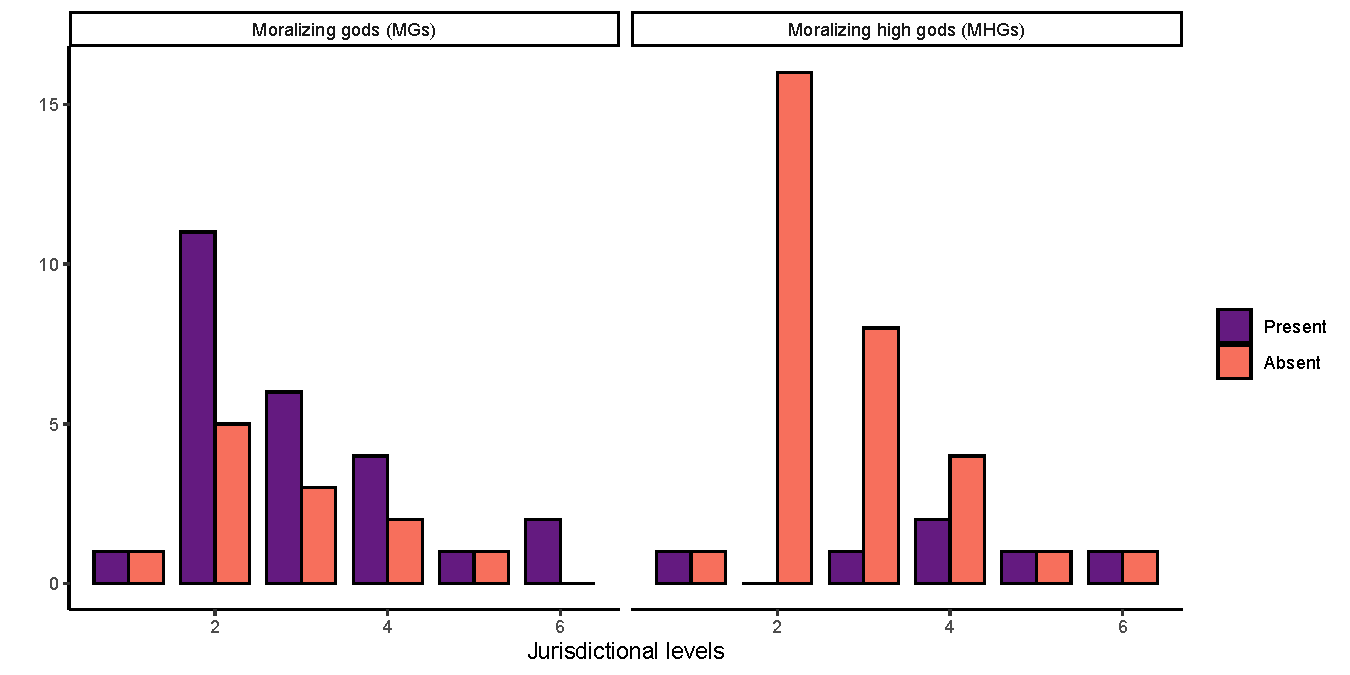
\includegraphics{mhg-writeup_files/figure-latex/compareSwanson-1.pdf}
\caption{\label{fig:compareSwanson}Number of MGs (left panel) and MHGs (right panel) that are coded as present vs.~absent in the Swanson (1964) dataset, where presence vs.~absence is assessed at the culture level. Cultures are grouped by jurisdictional levels, a proxy measure of social complexity (x-axis).}
\end{figure}

\begin{figure}
\centering
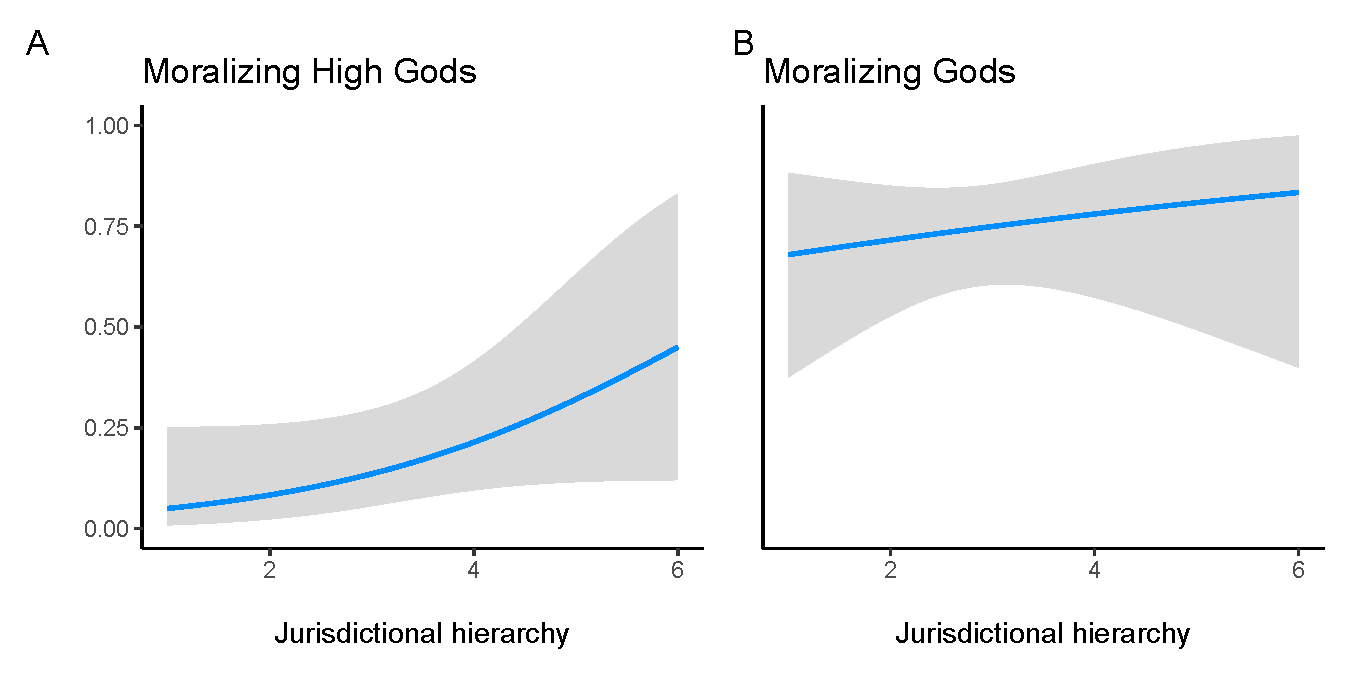
\includegraphics{mhg-writeup_files/figure-latex/compareSwansonMods-1.pdf}
\caption{\label{fig:compareSwansonMods}Logistic regression models showing the probability of a god present at the culture level (y-axis) as a function of social complexity, measured by the number of jurisdictional hierarchies (x-axis). A: When the god of interest is a MHG, we replicate the positive association with social complexity, discussed in the Introduction. B: When the god of interest is a MG, we see a higher prevalence of gods present and little-to-no association with social complexity.}
\end{figure}

Whereas figure \ref{fig:comparedatasets} shows that the use of MHGs to detect MGs creates many false negatives in the cross-cultural data, figures \ref{fig:compareSwanson} and \ref{fig:compareSwansonMods} suggest that those false negatives are not evenly distributed along levels of social complexity. Among cultures with lower levels of social complexity, there are many more claims of MHGs absent that are accompanied by cases of MGs present compared to the cultures with higher levels of social complexity. Put differently, the \emph{sensitivity} -- the true positive rate, or proportion of MGs correctly detected -- is biased, such that it increases with higher levels of social complexity (and, conversely, decreases with lower levels of social complexity).

We can create a simple model of this biased sensitivity, \(S\), as a function of social complexity level, \(SC\), where \(\text{logit}(S) = \alpha + \beta \times SC\). Here, \(\alpha\) is the intercept and \(\beta\) is the bias estimate along social complexity levels (see also Beesley and Mukherjee 2019). If \(\beta>0\), then the probability of correctly detecting a MG when one is present (\(S\)) increases as social complexity (\(SC\)) increases.

This biased sensitivity in our ability to detect MGs will clearly, to some extent, favor a positive association between MGs and social complexity. We approximate the extent to which this positive association is favored by estimating the parameters \(\alpha\) and \(\beta\) in the biased sensitivity model our available observations of MGs and MHGs along levels of social complexity. We do this using a bootstrap from Swanson's MHG and MG variables (\(N=10\,000\)), which shows the distribution of our estimates of \(\alpha\) and \(\beta\) in figure \ref{fig:swansonParameters}.\footnote{See our R script here: github link.}

\begin{figure}
\centering
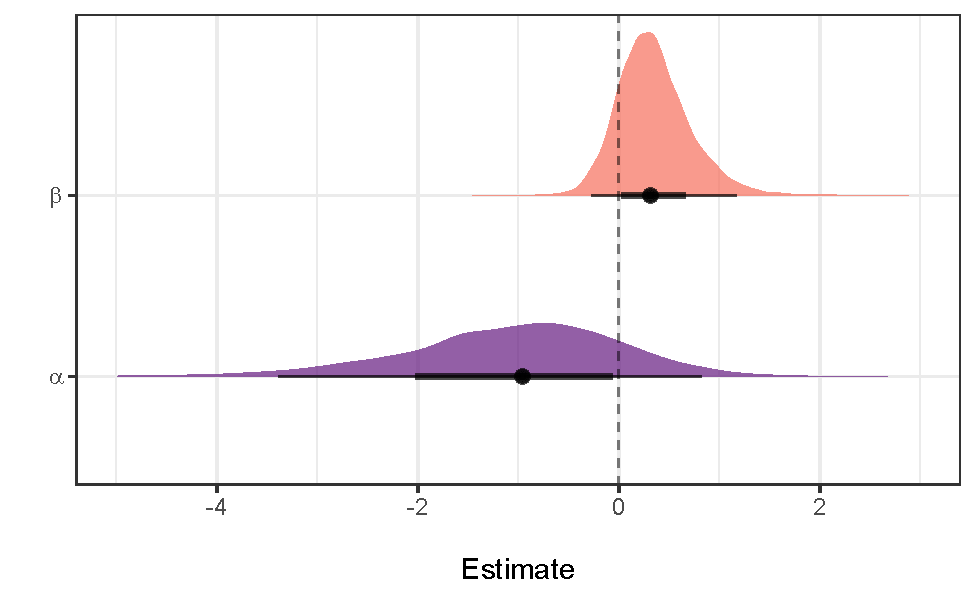
\includegraphics{mhg-writeup_files/figure-latex/swansonParameters-1.pdf}
\caption{\label{fig:swansonParameters}Distribution of parameters in our biased sensitivity model, from a bootstrapped sample of MHG and MG variables in Swanson (N=10,000).}
\end{figure}

Most of this range of biased sensitivity, where \(\beta>0\) and MGs tend to be more correctly detected at higher levels of social complexity, is sufficient to generate a spurious positive association between MGs and social complexity levels.

To demonstrate this, imagine that we could have a randomly generated ``population'' of, say, \(10\,000\) cultures. In this hypothetical world, there 74.5\% of the cultures have a MG present (the percentage of Swanson's cultures with a MG), and there is objectively no relationship between presence vs.~absence of MGs and social complexity, measured along five levels. Suppose we then sample 186 cultures from this population and observe false negatives from our biased sensitivity model, where \(P(\text{false negative}) = \text{logit}^{-1}(\alpha+\beta \times SC)\).\footnote{Similar to above, $SC$ is the level of social complexity and $\alpha$ and $\beta$ are the intercept and slope parameters, respectively, from the biased sensitivity inferred from the Swanson (1964) dataset} We can simulate this process many times (\(N=10\,000\) simulation runs), each time comparing the estimate from a logistic regression model based on perfect sensitivity -- where gods present are always accurately detected -- vs.~a logistic regression model based on our observations with biased false negatives. Perfect sensitivity unsurprisingly reflects the reality in our larger population (there is no relationship between social complexity and MGs). Our biased sensitivity model, however, reliably generates positive, ``statistically significant'' associations between social complexity and MGs (figure \ref{fig:biasedSimulation1}).

\begin{figure}
\centering
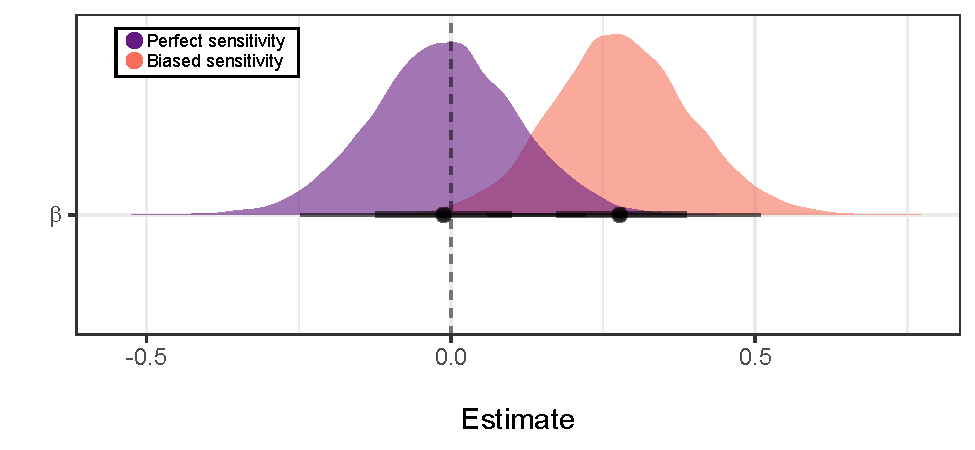
\includegraphics{mhg-writeup_files/figure-latex/biasedSimuation1-1.pdf}
\caption{\label{fig:biasedSimuation1}Distributions of estimates from logistic regression models of MGs as a function of social complexity, in a simulation where no relationship actually exists (N=10,000). Perfect sensitivity correctly infers no relationship (the purple distribution of estimates). Biased sensitivity, applying the average parameters from our bootstrap of the Swanson data to our biased sensitivity model, reliably generates a positive relationship (the orange distribution of estimates).}
\end{figure}

This simple exercise, which uses the available data on MGs and MHGs from Swanson (1964), shows that when we conceptualize the classification of MHGs in the data as error-prone attempts at detecting MGs in the cross-cultural data, we find a distribution of false negatives that can systematically favor a positive association between MGs and social complexity, even if none exists. Nevertheless, this proof of concept alone is not compelling, because the Swanson data is also a noisy and relatively small sample. The parameter distribution in figure \ref{fig:swansonParameters} is wide, and for simplicity, our simulation exercise was based on the average bias parameter, \(\beta\) from figure \ref{fig:compareSwansonMods} to generate false negatives in the simulation. It remains uncertain whether or not the simulation we have shown here actually captures the reality of the data-generating process in the MHG data. Perhaps our model, based on Swanson's data, overestimates the biased sensitivity of MG detection along social complexity levels as it exists in the SCCS.

As we will argue next, additional sources of bias in the data-generating process of the SCCS would have further contributed to generating a spurious association between MGs and social complexity. If anything, our biased sensitivity model likely \emph{under}estimates the bias, \(\beta\), that we inferred from Swanson's data.

\section{Biased false negatives in imperialist and missionary reports}\label{missionaries}

The debate about whether or not traditional populations lack MGs likely developed not as a scientific pursuit, but an imperial one in the form of missionization. Much of our knowledge or past traditional populations, including the sources that populate databases like the SCCS, come from missionaries and explorers who, in some cases, had explicitly biased their observations against the idea that moralizing religions could exist in small-scale societies.

{[}BGP section 3.1 on imperialist and missionary reports could go about here.{]}

Anthropologists during this time period had, in some cases, notably documented reams of evidence supporting the idea that traditional societies had religions. Tylor (1871), for example, extensively critiqued the idea that traditional, small-scale societies did not have religions, and developed his animistic theory of religion. Nevertheless, he simply dismisses the idea that small-scale religious traditions could have been moralistic in any way:

\begin{quote}
One great element of religion, that moral element which among the higher nations forms its most vital part, is indeed little represented in the religion of the lower races. It is not that these races have no moral sense or no moral standard, for both are strongly marked among them, if not in formal precept, at least in that traditional consensus of society which we call public opinion, according to which certain actions are held to be good or bad, right or wrong. It is that the conjunction of ethics and animistic philosophy, so intimate and powerful in the higher culture, seems scarcely yet to have begun in the lower (Tylor 1871/1920, p.~427).
\end{quote}

This rebuttal was an improvement on the prevailing assumption that small-scale societies had no religions. And yet, both sides of this debate stood in firm agreement in assuming that traditional small-scale societies had no MGs. This assumption was questioned a century later, when Evans-Pritchard, Evans-Pritchard, and Evans-Pritchard (1965) characterized the idea that traditional populations lack morally concerned gods as a myth. What revealed this sentiment as a myth was the effort of anthropologists who had conducted fieldwork among traditional populations. Anticipating what remains a common retort, Evans-Pritchard dismisses the presumption that simpler societies must have had to learn whatever moral elements in their religion from missionaries as ``condescending'' (Evans-Pritchard 1965; Hartland 1898; Lang 1909).

Among the sources used to code the MHG variable in the SCCS, 99.4\% (167 out of 168 societies with data on the presence of MHGs) are from \emph{before} Evans-Pritchard's defense of morally concerned gods among small-scale societies in 1965. The median year of these sources is 1920, and the vast majority (about 95\%) of sources were from pre-1950 (figure \ref{fig:sccsYearPlot}). Almost all of the data in the SCCS is therefore subject to the observational biases that prevailed during Tylor's time and beforehand, though it is worth noting that some, such as Malinowski, contested the idea that gods in small-scale societies lack moralistic concerns (for discussion, see Purzycki and McKay, forthcoming).

\begin{figure}
\centering
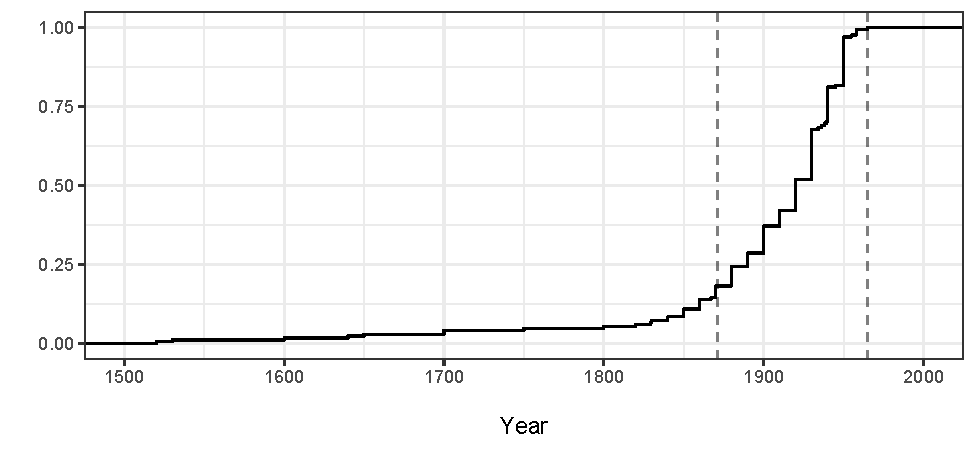
\includegraphics{mhg-writeup_files/figure-latex/sccsYearPlot-1.pdf}
\caption{\label{fig:sccsYearPlot}Empirical cumulative distribution function of the year of authorship for the records that code presence/absence of MHGs in the SCCS. For reference, the vertical lines highlight the years 1871 (the year Tylor first disputed the prevailing assumption that small-scale societies had no religions at all, shown to the left) and 1965 (the year Evans-Pritchard disputed the continuing trend of social scientists claiming that the gods of small-scale societies are not moralistic, shown to the right).}
\end{figure}

Hence, while it might be true that this prevailing view about MGs in small-scale societies did not shape all the ethnographies on which the SCCS high gods variable is based, there is good reason to assume that in many cases, it did. Not only would this have systematically underestimated the prevalence of MGs in the ethnographic record (figure \ref{fig:comparedatasets}), but this biased sensitivity along social complexity levels, as we demonstrated with a simple model and simulation, reliably generates a positive association between morally punitive gods and levels of social complexity.

\section{Moralizing gods in future research}

Many theories about the evolution of religion, such as the Big Gods narrative that we highlighted at the outset of this article, take as their premise that morally punitive gods are positively associated with large-scale societies. The evidence for this is, in large part, often based on analyses of cross-cultural and ethnographic data in the SCCS. The available measure that these studies use (presence/absence of MHGs) is meant to detect a theoretical construct that is frequently used interchangeably with Big Gods, but is unavailable in the SCCS (presence/absence of MGs).

We reviewed the coding criteria used for MHGs, and argued that these criteria systematically filter out MGs that are truly present. Specifically, is we assume that MHGs are a useful proxy measure for MGs, then the coding criteria for MHGs in the SCCS creates many false negatives because it includes a theoretically irrelevant filtering criteria: whether or not a deity is a creator deity, regardless of its omniscience, omnipotence, or its scope of concerns. This problem of false negatives is consistent with the observation that supernatural punishers are widespread in the ethnographic literature, including among small-scale hunter-gatherer societies (Boehm 2008).

In Swanson's smaller dataset that includes both MHGs and MGs, we find that this problem of false negatives (MHGs are ``absent,'' but MGs are ``present'') occurs non-randomly along levels of social complexity, such that cultures with low complexity were more likely to contain MHGs coded as ``absent'' and MGs coded as ``present.'' This bias, if it applies to the SCCS, would have likely suggested a spurious association between Big Gods and social complexity, but how likely this occurred for the SCCS depends on \emph{how biased} these false negatives were in the data-generating process. We used a simple model and the available data from Swanson (1964) to approximate this bias, and to show that it can reliably generate a positive association between MGs and social complexity (even when no such association actually exists). Swanson's dataset is relatively small and gives us a noisy inference to simulate from, but as we argued in section \ref{missionaries}, a review of the historical context in which the SCCS data were originally generated suggests that our assessment likely \emph{underestimates} this bias.

\begin{figure}
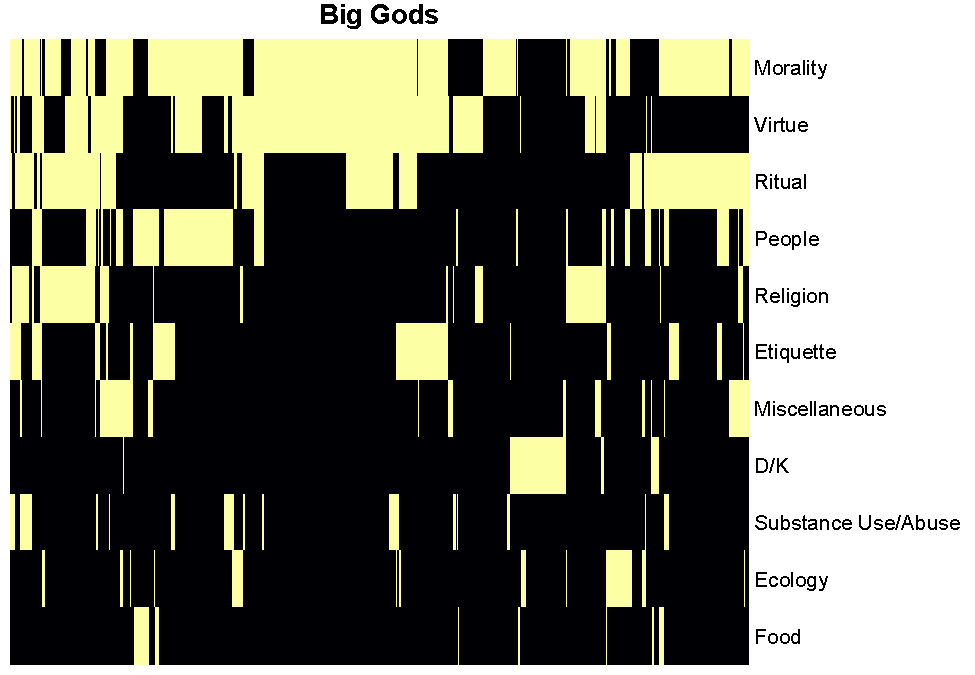
\includegraphics[width=0.5\linewidth]{mhg-writeup_files/figure-latex/bendixenPlot-1} 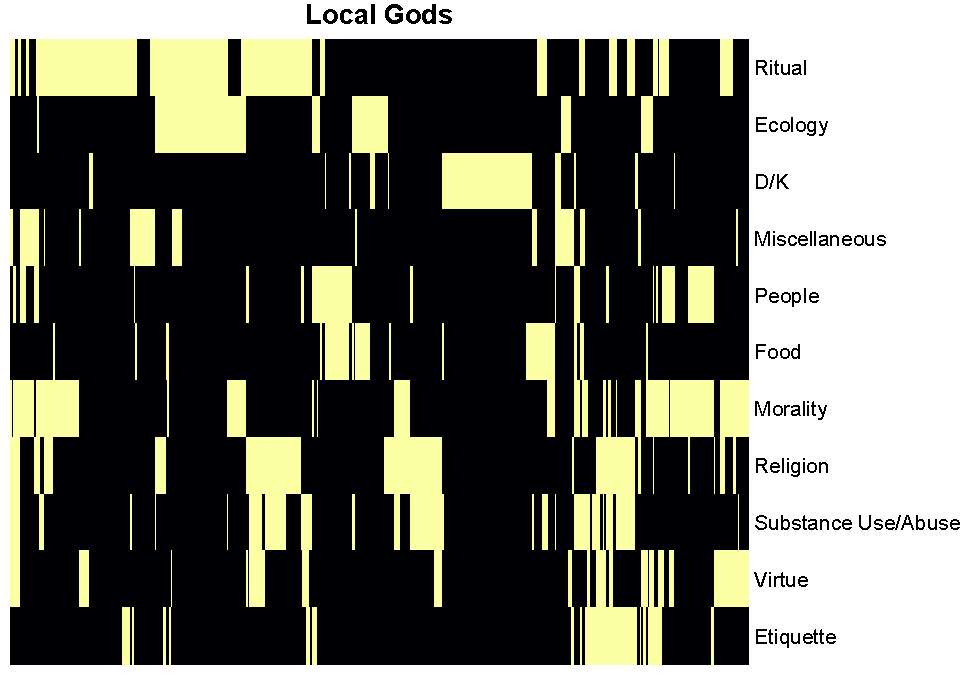
\includegraphics[width=0.5\linewidth]{mhg-writeup_files/figure-latex/bendixenPlot-2} \caption{Heatmap showing the presence (light cells) and absence (dark cells) of god concerns among eight cultures. Each column is a participant, and each rows is a domains that the participant responses were coded on. Data from Bendixen et al. (2021).}\label{fig:bendixenPlot}
\end{figure}

Given the arguments presented here, we question the prevailing assumption that a cross-cultural and historical association exists between punitive MGs and social complexity. While it can be beneficial to reject a misleading assumption, this is only the first step going forward. Cross-cultural ethnographic work relying not on coding ethnographers' observations, but on actively asking participants to provide descriptions of their moralizing gods, has only recently begun (Purzycki et al. 2016; Lang et al. 2019; e.g., Bendixen et al. 2021; Singh, Kaptchuk, and Henrich 2021).

In individual-level data collected across eight cultures by Purzycki et al. (2016), many people claimed that moralizing gods were concerned about interpersonal behavior, among a wide range of other social and ecological domains of concern (see also Bendixen et al. 2021). The domains of these gods' concerns tend to vary among the gods designated as ``big gods'' and ``local gods'' -- a distinction whose usefulness might vary in different cultural contexts (Placek and Lightner 2022) -- and they also vary among different gods we find in different socioecological contexts (figure \ref{fig:bendixenPlot}; see also Purzycki and McNamara (2016)). Importantly, the participants in Purzycki et al.~also usually claimed to believe in supernatural punishment, regardless of how ``big'' the gods in question were (83\% believed in punitive big gods, and 75\% believed in punitive local gods).

Questions surrounding supernatural punishers have come a long way since questions about their existence throughout much of the early twentieth century. As evidence accumulates in support of their cross-cultural existence, contra Tylor and his contemporary critics, it is imperative that we also reassess the cross-cultural datasets whose formation was shaped by outdated theories (Bendixen and Purzycki 2020; Bendixen, Lightner, and Purzycki 2021; Lightner and Purzycki 2021). Ethnographic work is needed now more than ever, but it must be informed going forward by theories that are not burdened by centuries-old sets of assumptions.

\section*{Acknowledgements}

All authors thank the Aarhus University Research Foundation for support.

\section*{References}

\hypertarget{refs}{}
\begin{CSLReferences}{1}{0}
\leavevmode\hypertarget{ref-beesleyStatisticalInferenceAssociation2019}{}%
Beesley, Lauren J., and Bhramar Mukherjee. 2019. \emph{Statistical Inference for Association Studies Using Electronic Health Records: Handling Both Selection Bias and Outcome Misclassification}.

\leavevmode\hypertarget{ref-beheimCorrectedAnalysesShow2019}{}%
Beheim, Bret, Quentin Atkinson, Joseph Bulbulia, Will Gervais, Russell Gray, Joseph Henrich, Martin Lang, M. Monroe, Michael Muthukrishna, Ara Norenzayan, Benjamin Purzycki, Azim Shariff, Edward Slingerland, Rachel Spicer, and Aiyana Willard. 2019. \emph{Corrected Analyses Show That Moralizing Gods Precede Complex Societies but Serious Data Concerns Remain}.

\leavevmode\hypertarget{ref-bendixenAppealingMindsGods2021}{}%
Bendixen, Theiss, Coren Apicella, Quentin Atkinson, Emma Cohen, Joseph Henrich, Rita Anne McNamara, Ara Norenzayan, Aiyana Willard, Dimitris Xygalatas, and Benjamin Grant Purzycki. 2021. \emph{Appealing to the Minds of Gods: {A} Novel Cultural Evolutionary Account of Religious Appeals and an Empirical Assessment Using Ethnographic Data from Eight Diverse Societies}. PsyArXiv.

\leavevmode\hypertarget{ref-bendixenCulturalEvolutionReligion2021}{}%
Bendixen, Theiss, Aaron Lightner, and Benjamin Grant Purzycki. 2021. \emph{The {Cultural} {Evolution} of {Religion} and {Cooperation}}. PsyArXiv.

\leavevmode\hypertarget{ref-bendixenPeeringMindsGods2020}{}%
Bendixen, Theiss, and Benjamin Purzycki. 2020. {``Peering into the {Minds} of {Gods}: {What} {Cross}-{Cultural} {Variation} in {Gods}' {Concerns} {Can} {Tell} {Us} about the {Evolution} of {Religion}.''} \emph{Journal for the Cognitive Science of Religion}. doi: \href{https://doi.org/10.1558/jcsr.40951}{10.1558/jcsr.40951}.

\leavevmode\hypertarget{ref-boehm2008biocultural}{}%
Boehm, Christopher. 2008. {``A Biocultural Evolutionary Exploration of Supernatural Sanctioning.''} \emph{Evolution of Religion: Studies, Theories, and Critiques} 143--52.

\leavevmode\hypertarget{ref-duffy2004simple}{}%
Duffy, SW, J. Warwick, ARW Williams, H. Keshavarz, F. Kaffashian, TE Rohan, F. Nili, and A. Sadeghi-Hassanabadi. 2004. {``A Simple Model for Potential Use with a Misclassified Binary Outcome in Epidemiology.''} \emph{Journal of Epidemiology \& Community Health} 58(8):712--17.

\leavevmode\hypertarget{ref-edwards2013accounting}{}%
Edwards, Jessie K., Stephen R. Cole, Melissa A. Troester, and David B. Richardson. 2013. {``Accounting for Misclassified Outcomes in Binary Regression Models Using Multiple Imputation with Internal Validation Data.''} \emph{American Journal of Epidemiology} 177(9):904--12.

\leavevmode\hypertarget{ref-evans-pritchardTheoriesPrimitiveReligion1965}{}%
Evans-Pritchard, Edward Evan, Edward Evans Evans-Pritchard, and Sir Edward Evans-Pritchard. 1965. \emph{Theories of {Primitive} {Religion}}. Clarendon Press.

\leavevmode\hypertarget{ref-fitouchiSupernaturalPunishmentBeliefs2021}{}%
Fitouchi, Léo, and Manvir Singh. 2021. {``Supernatural Punishment Beliefs as Cognitively Compelling Tools of Social Control.''} \emph{Current Opinion in Psychology} 44:252--57. doi: \href{https://doi.org/10.1016/j.copsyc.2021.09.022}{10.1016/j.copsyc.2021.09.022}.

\leavevmode\hypertarget{ref-henrichOriginsPsychologyHuman2021}{}%
Henrich, Joseph, and Michael Muthukrishna. 2021. {``The {Origins} and {Psychology} of {Human} {Cooperation}.''} \emph{Annual Review of Psychology} 72(1):207--40. doi: \href{https://doi.org/10.1146/annurev-psych-081920-042106}{10.1146/annurev-psych-081920-042106}.

\leavevmode\hypertarget{ref-jacksonTightCulturesVengeful2021}{}%
Jackson, Joshua Conrad, Nava Caluori, Samantha Abrams, Elizabeth Beckman, Michele Gelfand, and Kurt Gray. 2021. {``Tight Cultures and Vengeful Gods: {How} Culture Shapes Religious Belief.''} \emph{Journal of Experimental Psychology: General} No Pagination Specified--. doi: \href{https://doi.org/10.1037/xge0001033}{10.1037/xge0001033}.

\leavevmode\hypertarget{ref-johnsonGodWatchingYou2015}{}%
Johnson, Dominic. 2015. \emph{God {Is} {Watching} {You}: {How} the {Fear} of {God} {Makes} {Us} {Human}}. 1 edition. New York: Oxford University Press.

\leavevmode\hypertarget{ref-johnsonGodPunishmentPublic2005}{}%
Johnson, Dominic D. P. 2005. {``God's Punishment and Public Goods : {A} Test of the Supernatural Punishment Hypothesis in 186 World Cultures.''} \emph{Human Nature (Hawthorne, N.Y.)} 16(4):410--46. doi: \href{https://doi.org/10.1007/s12110-005-1017-0}{10.1007/s12110-005-1017-0}.

\leavevmode\hypertarget{ref-kirbyDPLACEGlobalDatabase2016}{}%
Kirby, Kathryn R., Russell D. Gray, Simon J. Greenhill, Fiona M. Jordan, Stephanie Gomes-Ng, Hans-Jörg Bibiko, Damián E. Blasi, Carlos A. Botero, Claire Bowern, Carol R. Ember, Dan Leehr, Bobbi S. Low, Joe McCarter, William Divale, and Michael C. Gavin. 2016. {``D-{PLACE}: {A} {Global} {Database} of {Cultural}, {Linguistic} and {Environmental} {Diversity}''} edited by A. Mesoudi. \emph{PLOS ONE} 11(7):e0158391. doi: \href{https://doi.org/10.1371/journal.pone.0158391}{10.1371/journal.pone.0158391}.

\leavevmode\hypertarget{ref-langMoralizingGodsImpartiality2019}{}%
Lang, Martin, Benjamin G. Purzycki, Coren L. Apicella, Quentin D. Atkinson, Alexander Bolyanatz, Emma Cohen, Carla Handley, Eva Kundtová Klocová, Carolyn Lesorogol, Sarah Mathew, Rita A. McNamara, Cristina Moya, Caitlyn D. Placek, Montserrat Soler, Thomas Vardy, Jonathan L. Weigel, Aiyana K. Willard, Dimitris Xygalatas, Ara Norenzayan, and Joseph Henrich. 2019. {``Moralizing Gods, Impartiality and Religious Parochialism Across 15 Societies.''} \emph{Proceedings of the Royal Society B: Biological Sciences} 286(1898):20190202. doi: \href{https://doi.org/10.1098/rspb.2019.0202}{10.1098/rspb.2019.0202}.

\leavevmode\hypertarget{ref-lightnerGameTheoreticalAspects2021}{}%
Lightner, Aaron, and Benjamin Grant Purzycki. 2021. \emph{Game {Theoretical} {Aspects} of the {Minds} of {Gods}}. PsyArXiv.

\leavevmode\hypertarget{ref-murdockStandardCrossCulturalSample2006}{}%
Murdock, George P., and Douglas R. White. 2006. {``Standard {Cross}-{Cultural} {Sample}: On-Line Edition.''}

\leavevmode\hypertarget{ref-norenzayanBigGodsHow2015}{}%
Norenzayan, Ara. 2015. \emph{Big {Gods}: {How} {Religion} {Transformed} {Cooperation} and {Conflict}}. Reprint edition. Princeton Oxford: Princeton University Press.

\leavevmode\hypertarget{ref-norenzayanCulturalEvolutionProsocial2016}{}%
Norenzayan, Ara, Azim F. Shariff, Will M. Gervais, Aiyana K. Willard, Rita A. McNamara, Edward Slingerland, and Joseph Henrich. 2016. {``The Cultural Evolution of Prosocial Religions.''} \emph{Behavioral and Brain Sciences} 39:e1. doi: \href{https://doi.org/10.1017/S0140525X14001356}{10.1017/S0140525X14001356}.

\leavevmode\hypertarget{ref-peoplesHunterGatherersOriginsReligion2016}{}%
Peoples, Hervey C., Pavel Duda, and Frank W. Marlowe. 2016. {``Hunter-{Gatherers} and the {Origins} of {Religion}.''} \emph{Human Nature} 27(3):261--82. doi: \href{https://doi.org/10.1007/s12110-016-9260-0}{10.1007/s12110-016-9260-0}.

\leavevmode\hypertarget{ref-peoplesSubsistenceEvolutionReligion2012}{}%
Peoples, Hervey, and Frank Marlowe. 2012. {``Subsistence and the {Evolution} of {Religion}.''} \emph{Human Nature (Hawthorne, N.Y.)} 23:253--69. doi: \href{https://doi.org/10.1007/s12110-012-9148-6}{10.1007/s12110-012-9148-6}.

\leavevmode\hypertarget{ref-peregrineBirthGodsRevisited1996}{}%
Peregrine, Peter. 1996. {``The {Birth} of the {Gods} {Revisited}: {A} {Partial} {Replication} of {Guy} {Swanson}'s (1960) {Cross}-{Cultural} {Study} of {Religion}.''} \emph{Cross-Cultural Research} 30(1):84--112. doi: \href{https://doi.org/10.1177/106939719603000104}{10.1177/106939719603000104}.

\leavevmode\hypertarget{ref-purzyckiEcologicalTheoryGods2016}{}%
Purzycki, Benjamin G., and Rita A. McNamara. 2016. {``An {Ecological} {Theory} of {Gods}' {Minds}.''} in \emph{Advances in religion, cognitive science, and experimental philosophy, {Ed}. {Helen} {DeCruz}}. New York: Bloomsbury.

\leavevmode\hypertarget{ref-purzyckiMoralisticGodsSupernatural2016}{}%
Purzycki, Benjamin Grant, Coren Apicella, Quentin D. Atkinson, Emma Cohen, Rita Anne McNamara, Aiyana K. Willard, Dimitris Xygalatas, Ara Norenzayan, and Joseph Henrich. 2016. {``Moralistic Gods, Supernatural Punishment and the Expansion of Human Sociality.''} \emph{Nature} 530(7590):327--30. doi: \href{https://doi.org/10.1038/nature16980}{10.1038/nature16980}.

\leavevmode\hypertarget{ref-roesBeliefMoralizingGods2003}{}%
Roes, Frans L., and Michel Raymond. 2003. {``Belief in Moralizing Gods.''} \emph{Evolution and Human Behavior} 24(2):126--35. doi: \href{https://doi.org/10.1016/S1090-5138(02)00134-4}{10.1016/S1090-5138(02)00134-4}.

\leavevmode\hypertarget{ref-schlossEvolutionaryAccountsBelief2011}{}%
Schloss, Jeffrey P., and Michael J. Murray. 2011. {``Evolutionary Accounts of Belief in Supernatural Punishment: A Critical Review.''} \emph{Religion, Brain \& Behavior} 1(1):46--99. doi: \href{https://doi.org/10.1080/2153599X.2011.558707}{10.1080/2153599X.2011.558707}.

\leavevmode\hypertarget{ref-singhSmallGodsRituals2021}{}%
Singh, Manvir, Ted J. Kaptchuk, and Joseph Henrich. 2021. {``Small Gods, Rituals, and Cooperation: {The} {Mentawai} Water Spirit {Sikameinan}.''} \emph{Evolution and Human Behavior} 42(1):61--72. doi: \href{https://doi.org/10.1016/j.evolhumbehav.2020.07.008}{10.1016/j.evolhumbehav.2020.07.008}.

\leavevmode\hypertarget{ref-skoggard2020resource}{}%
Skoggard, Ian, Carol R. Ember, Emily Pitek, Joshua Conrad Jackson, and Christina Carolus. 2020. {``Resource Stress Predicts Changes in Religious Belief and Increases in Sharing Behavior.''} \emph{Human Nature} 31(3):249--71.

\leavevmode\hypertarget{ref-snareyNaturalEnvironmentImpact1996}{}%
Snarey, John. 1996. {``The {Natural} {Environment}'s {Impact} Upon {Religious} {Ethics}: {A} {Cross}-{Cultural} {Study}.''} \emph{Journal for the Scientific Study of Religion} 35(2):85--96. doi: \href{https://doi.org/10.2307/1387077}{10.2307/1387077}.

\leavevmode\hypertarget{ref-swansonBirthGods1964}{}%
Swanson, Guy. 1964. \emph{The {Birth} of the {Gods}}.

\leavevmode\hypertarget{ref-tylorPrimitiveCultureResearches1871}{}%
Tylor, Edward Burnett. 1871. \emph{Primitive {Culture}: {Researches} into the {Development} of {Mythology}, {Philosophy}, {Religion}, {Art}, and {Custom}}. Vol. 2. Cambridge: Cambridge University Press.

\leavevmode\hypertarget{ref-wattsBroadSupernaturalPunishment2015}{}%
Watts, Joseph, Simon J. Greenhill, Quentin D. Atkinson, Thomas E. Currie, Joseph Bulbulia, and Russell D. Gray. 2015. {``Broad Supernatural Punishment but Not Moralizing High Gods Precede the Evolution of Political Complexity in {Austronesia}.''} \emph{Proceedings. Biological Sciences} 282(1804):20142556. doi: \href{https://doi.org/10.1098/rspb.2014.2556}{10.1098/rspb.2014.2556}.

\leavevmode\hypertarget{ref-whitehouseBigGodsDid2021}{}%
Whitehouse, Harvey, Pieter François, Patrick E. Savage, Daniel Hoyer, Kevin C. Feeney, Enrico Cioni, Rosalind Purcell, Robert M. Ross, Jennifer Larson, John Baines, Barend ter Haar, Alan Covey, and Peter Turchin. 2021. \emph{Big {Gods} Did Not Drive the Rise of Big Societies Throughout World History}. OSF Preprints.

\end{CSLReferences}

\end{document}
